\documentclass[a4j]{celb-report}
%%%
%%% 計算機工学実験Bレポートテンプレート
%%%  このテンプレートを使う場合,celb-report.clsとjlisting.styが必要です.
%%%  このファイルと同じディレクトリに置いておいてください.
%%%

%%%
%%% まずはここで各種設定
%%%
\usepackage{comment}
\period{2} % ← 何回目のレポートか(1~3)
\stunum{学籍番号} % ← 学生番号
\author{伊藤太清} % ← 学生氏名
\date{\today} % ← レポート提出日

\begin{document}

\maketitle

%%%%%%%%%%%%%%%%%%%%%%%%%%%%%%%%%%%%%%%%%%%%%%%%%%%%%%%%%%%%%%%%%%%%%
% レポート作成の手引:
%   レポート提出時は、ここから「レポート作成の手引ここまで」までの行をすべて削除すること!
%%%%%%%%%%%%%%%%%%%%%%%%%%%%%%%%%%%%%%%%%%%%%%%%%%%%%%%%%%%%%%%%%%%%%
\begin{comment}
\setcounter{section}{-1}
\section{レポート作成の手引}

各レポート,対応する回ごとに章(\verb|\section|)に分け,テキストの報告内容にて指示されている課題ごとに節(\verb|\subsection|)を用意して記載する.次章にて第1回分の例を記載しているので,適宜参考にすること.

% ----------------------------------------------------
\subsection{プログラムのソースコード,実行結果等を掲載する場合}

プログラムのソースコードや実行結果等を貼り付ける場合は,\verb|\lstlisting|環境を用いると良い.使い方は,このファイルの\texttt{tex}ソースを参考にすること.基本的には,ソースに記載の内容をコピーし,実行結果を書き換えると良い.
%
% --- 実行結果ここから
\begin{lstlisting}[basicstyle=\ttfamily\footnotesize, frame=single]

※※ ここに実行結果を貼り付ける. ※※
 
\end{lstlisting}
% --- 実行結果ここまで
%

% ----------------------------------------------------
\subsection{課題}

各回で用意されている考察・調査課題については,\verb|\kadai|を用いて,課題文と回答を記載する.第1回分の例を参考にすること.

% ----------------------------------------------------
\subsection{図の貼り付け}

図を貼り付ける場合は,\verb|\figure|環境を用いる.基本的には,このファイルの\texttt{tex}ソース内にある記述をそのまま用いれば良い.\verb|\includegraphcs|で画像ファイルを指定し,\verb|\caption|で図にキャプションを付ける.\verb|\label|は,本文中で図番号を参照するために付けておくラベルである(詳しくは後述).
%
\begin{figure}[htb]
 \centering 
\includegraphics[scale=0.8]{sample-figure.eps}
 \caption{図のサンプル} \label{fig:sample}
\end{figure}
%

本文中で図を引用する場合は,図中で指定した\verb|label|を\verb|\ref|を用いて参照する.例えば上図で\verb|\label{fig:sample}|としている状態で本文中に``図\verb|\ref{fig:sample}|''と記述すると,texコンパイル後のファイルでは当該箇所が``図\ref{fig:sample}''に変換される.``図??''となる場合は,もう1度texコンパイルしてみて,それでも参照がされない場合は,ラベルが一致しているかどうか確認する.

% ----------------------------------------------------
\subsection{(第3レポートのみ)グループ内の役割分担}

第3レポートの対象となる回では,複数人のグループで作業を行うため,各回で誰が何を担当したのかも節(\verb|\subsection|)を用いて記載する.以下は記載例である.\texttt{tex}ソースに記載の通り,\verb|\description|環境を用いると良い.
%
\begin{description}
 \item[s123456 学生 なまえ] ネットワークの配線,環境の構築
 \item[s135791 相方 ひとりめ] プログラムのコーディング,デバッグ
 \item[s246802 相方 ふたりめ] コーディングのサポート
 \item[s369258 相方 さんにんめ] 3人の応援
\end{description}

% ----------------------------------------------------
\subsection{参考文献等}

書籍,インターネット上の情報などを参考にした場合,対象となるすべての回のものをまとめて,\verb|\thebibliography|環境を用いて出展を明記する.書き方は本ファイルの\texttt{tex}ソースを参考にする.
%
%%%%%%%%%%%%%%%%%%%%%%%%%%%%%%%%%%%%%%%%%%%%%%%%%%%%%%%%%%%%%%%%%%%%%
% レポート作成の手引ここまで
%%%%%%%%%%%%%%%%%%%%%%%%%%%%%%%%%%%%%%%%%%%%%%%%%%%%%%%%%%%%%%%%%%%%%


%%%%%%%%%%%%%%%%%%%%%%%%%%%%%%%%%%%%%%%%%%%%%%%%%%%%%%%%%%%%%%%%%%%%%
% 第1回分(第1レポート内)サンプル
%   第1レポートでは,第1回~第4回分それぞれを 章 (\section) として1つのレポートにまとめること
%%%%%%%%%%%%%%%%%%%%%%%%%%%%%%%%%%%%%%%%%%%%%%%%%%%%%%%%%%%%%%%%%%%%%
%%% ------------------------------------------------------------------
\newpage % ← 改ページ
\section{第1回 誤り制御符号(1):パリティ符号}

% ----------------------------------------------------
\subsection{実行結果}

%
% --- 実行結果ここから
\begin{lstlisting}[basicstyle=\ttfamily\footnotesize, frame=single]
$ ./parity



...


 
\end{lstlisting}
% --- 実行結果ここまで
%

\subsection{実行結果に対する考察}
前節の実行結果より,~であることがわかる.また,~であるものと考えられる.


% ----------------------------------------------------
\subsection{課題}

\kadai{今回の実験で作成したパリティ符号は,偶数パリティと奇数パリティのいずれであるかを答えよ.}

~~~であるため,◯数パリティである.

\kadai{1ビット水平パリティ符号について調査せよ.}

1ビット水平パリティ符号とは,~~ものである.~~.

\kadai{1ビット水平パリティ符号と1ビット垂直パリティ符号を組み合わせることにより,1ビットの誤りを訂正できることを示せ.}

~~.

以上より,1ビット水平パリティ符号と~~~,~~~できる.
\end{comment}
%
%%%%%%%%%%%%%%%%%%%%%%%%%%%%%%%%%%%%%%%%%%%%%%%%%%%%%%%%%%%%%%%%%%%%%
% 第1回分サンプルここまで
%%%%%%%%%%%%%%%%%%%%%%%%%%%%%%%%%%%%%%%%%%%%%%%%%%%%%%%%%%%%%%%%%%%%%

%%% ------------------------------------------------------------------
\section{第5回 TPCソケットの基礎}
\subsection{プログラムの実行結果}
ECHOクライアントを実行した結果は以下のようになった。
\begin{lstlisting}[basicstyle=\ttfamily\footnotesize, frame=single]
10.232.30.7000
Connect to 10.210.232.30:7000 ...
Socket is connected...
SEND>> cel-B
RECIEVE>> cel-B
SEND>> cel-B
RECIEVE>> cel-B
SEND>> cel-B
RECIEVE>> cel-B
SEND>> ^C
\end{lstlisting}
\begin{comment}
\begin{figure}[htb]
 \centering
 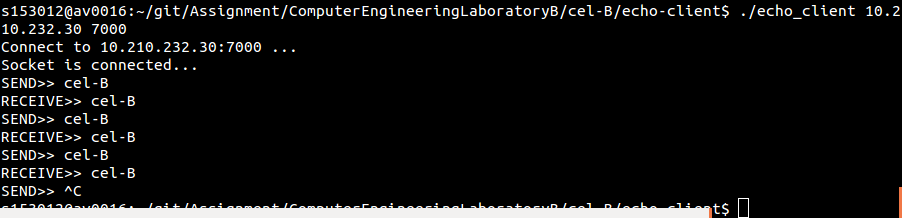
\includegraphics[width=15cm]{../echo-client/echo_client_output.png}
 \caption{echo\_client実行結果} \label{EchoClientOutput}
\end{figure}
\end{comment}
\subsection{プログラムの改造}
クライアントがrecvコマンドで文字列を受け取ったあと、表示する際に、戻ってきた長さを表示するように改造したecho\_client2の実行結果は以下のようになった。
\begin{lstlisting}[basicstyle=\ttfamily\footnotesize, frame=single]
Connect to 10.210.232.137:7000 ...
Socket is connected...
SEND>> cel-B
RECIEVE>> cel-B (5)
SEND>> abc
RECIEVE>> abc (3)
SEND>> qwerty
RECIEVE>> qwerty (6)
SEND>> ^C
\end{lstlisting}
\begin{comment}
\begin{figure}[htb]
 \centering
 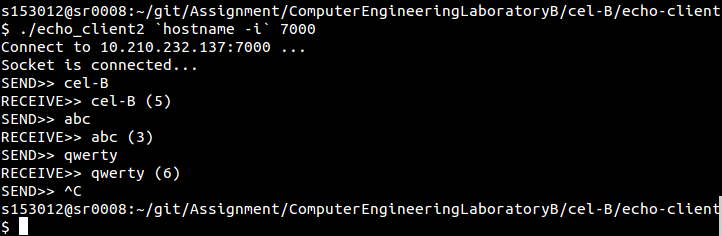
\includegraphics[width=15cm]{../echo-client/echo_client2_output.png}
 \caption{echo\_client2実行結果} \label{EchoClient2Output}
\end{figure}
\end{comment}
\subsection{調査課題}
\begin{enumerate}
 \renewcommand{\labelenumi}{(\arabic{enumi})}
 \item 今回のプログラム中で使用されている connect 関数の仕様について調査し, echo\_client.c 中での使用例を書き出し,どのような動作を意図しているかを説明せよ.\\
\\
92行目、93行目で以下のようにconnect関数が使われている。
  \begin{lstlisting}[basicstyle=\ttfamily\footnotesize, frame=single]
    status = connect(destSocket, (struct sockaddr *)&destSockAddr, 
                    (socklen_t)sizeof(destSockAddr));
  \end{lstlisting}
  \begin{itemize}
   \item 機能:ソケットで接続を確立する。
   \item 引数\\
destSockedは接続に使うソケットのディスクリプタ\\
(struct sockaddr *)\&destSocketAddrは接続先のIPアドレスとポート番号が入ったsockaddr構造体へのポインタ\\
(socklen\_t)sizeof(destSockAddr)はsockaddr構造体のサイズ
   \item 返り値:成功した時0を、失敗した時-1を返す。
  \end{itemize}
 \item 今回のプログラム中で使用されている recv 関数の仕様について調査し, echo\_client.c 中での使用例を書き出し, どのような動作を意図しているかを説明せよ.\\
\\
134行目で以下のようにrecv関数が使われている。
  \begin{lstlisting}[basicstyle=\ttfamily\footnotesize, frame=single]
        numrcv = recv(destSocket, recvStr, BUFFER_LEN, NO_FLAGS_SET);
  \end{lstlisting}
  \begin{itemize}
   \item 機能:メッセージを受信する。
   \item 引数\\
destSocketは受信に使うソケットのディスクリプタ\\
recvStrは受信したデータを受け取るアドレス\\
BUFFER\_LENはメッセージの最大バイト数\\
NO\_FLAGS\_SETはソケットが呼びだされた際の動作を指定する。NO\_FLAGS\_SETはデフォルトの動作
   \item 返り値:成功した時受信したバイト数を、失敗した時-1を返す。
  \end{itemize}
\end{enumerate}


%%% ------------------------------------------------------------------
\newpage
\section{第6回 ECHOサーバの作成}
\subsection{プログラムの実行結果}
echo\_server.cをコピーしてコンパイルして実行させ、別のターミナルを開いて前回のecho\_clientを実行させたところ、サーバ側とクライアント側でそれぞれ以下のような実行結果を得た。
%server-output
\begin{lstlisting}[caption=サーバ側実行結果, basicstyle=\ttfamily\footnotesize, frame=single]
Waiting for connection ...
Connected from 10.210.232.48.
RECIEVE(4)>>abc
RECIEVE(4)>>def
RECIEVE(4)>>ghi
Connection terminated
Waiting for connection ...
Connected from 10.210.232.48.
RECIEVE(4)>>jkl
RECIEVE(4)>>mno
RECIEVE(4)>>pqr
Connection terminated
Waiting for connection ...
Connected from 10.210.232.48.
RECIEVE(4)>>stu
RECIEVE(4)>>vwx
RECIEVE(3)>>yx
Connection terminated
Waiting for connection ...
^C
\end{lstlisting}
%client-output
\begin{lstlisting}[caption=クライアント側実行結果1, basicstyle=\ttfamily\footnotesize, frame=single]
Connect to 10.210.232.48:7000 ...
Socket is connected...
SEND>> abc
RECIEVE>> abc
SEND>> def
RECIEVE>> def
SEND>> ghi
RECIEVE>> ghi
SEND>> ^c
\end{lstlisting}
\begin{lstlisting}[caption=クライアント側実行結果2, basicstyle=\ttfamily\footnotesize, frame=single]
Connect to 10.210.232.48:7000 ...
Socket is connected...
SEND>> jkl
RECIEVE>> jkl
SEND>> mno
RECIEVE>> mno
SEND>> pqr
RECIEVE>> pqr
SEND>> ^c
\end{lstlisting}
\begin{lstlisting}[caption=クライアント側実行結果3, basicstyle=\ttfamily\footnotesize, frame=single]
Connect to 10.210.232.48:7000 ...
Socket is connected...
SEND>> stu
RECIEVE>> stu
SEND>> vwx
RECIEVE>> vwx
SEND>> yz
RECIEVE>> yz
SEND>> ^c
\end{lstlisting}
別の計算機上でサーバを起動させクライアント側でそこに接続した場合も、同様に以下のような実行結果が得られた。
%server-output2
\begin{lstlisting}[caption=サーバ側実行結果, basicstyle=\ttfamily\footnotesize, frame=single]
Waiting for connection ...
Connected from 10.210.232.47.
RECIEVE(4)>>abc
RECIEVE(4)>>def
RECIEVE(4)>>ghi
Connection terminated
Waiting for connection ...
Connected from 10.210.232.47.
RECIEVE(4)>>jkl
RECIEVE(4)>>mno
RECIEVE(4)>>pqr
Connection terminated
Waiting for connection ...
Connected from 10.210.232.47.
RECIEVE(4)>>stu
RECIEVE(4)>>vwx
RECIEVE(3)>>yx
Connection terminated
Waiting for connection ...
^C
\end{lstlisting}
%client-output2
\begin{lstlisting}[caption=クライアント側実行結果1, basicstyle=\ttfamily\footnotesize, frame=single]
Connect to 10.210.232.48:7000 ...
Socket is connected...
SEND>> abc
RECIEVE>> abc
SEND>> def
RECIEVE>> def
SEND>> ghi
RECIEVE>> ghi
SEND>> ^c
\end{lstlisting}
\begin{lstlisting}[caption=クライアント側実行結果2, basicstyle=\ttfamily\footnotesize, frame=single]
Connect to 10.210.232.48:7000 ...
Socket is connected...
SEND>> jkl
RECIEVE>> jkl
SEND>> mno
RECIEVE>> mno
SEND>> pqr
RECIEVE>> pqr
SEND>> ^c
\end{lstlisting}
\begin{lstlisting}[caption=クライアント側実行結果3, basicstyle=\ttfamily\footnotesize, frame=single]
Connect to 10.210.232.48:7000 ...
Socket is connected...
SEND>> stu
RECIEVE>> stu
SEND>> vwx
RECIEVE>> vwx
SEND>> yz
RECIEVE>> yz
SEND>> ^c
\end{lstlisting}
\subsection{プログラムの改造}
ECHO サーバから send コマンドで文字列を送り返すとき,クライアントから送られたきた文字列を,最初の 1 文字ですべて置き換えた文字列に直して送り返すように改造したプログラム echo server2 を作成し、コンパイルしてサーバとクライアントを実行したところ、以下のような実行結果が得られた。
%server-output3
\begin{lstlisting}[caption=サーバ側実行結果, basicstyle=\ttfamily\footnotesize, frame=single]
Waiting for connection ...
Connected from 10.210.232.48.
RECIEVE(4)>>abc
RECIEVE(6)>>cel-B
RECIEVE(7)>>qwerty
Connection terminated
Waiting for connection ...
^C
\end{lstlisting}
%client-output3
\begin{lstlisting}[caption=クライアント側実行結果, basicstyle=\ttfamily\footnotesize, frame=single]
Connect to 10.210.232.48:7000 ...
Socket is connected...
SEND>> abc
RECIEVE>> aaa
SEND>> cel-B
RECIEVE>> ccccc
SEND>> qwerty
RECIEVE>> qqqqqq
SEND>> ^c
\end{lstlisting}
\subsection{加点課題}
クライアントから送られて来た文字列を逆順に並べて送り返すように改造したプログラム echo server3 を作成し、コンパイルしてサーバとクライアントを実行したところ、以下のような実行結果が得られた。
%server-output4
\begin{lstlisting}[caption=サーバ側実行結果, basicstyle=\ttfamily\footnotesize, frame=single]
Waiting for connection ...
Connected from 10.210.232.48.
RECIEVE(4)>>abc
RECIEVE(6)>>cel-B
RECIEVE(7)>>qwerty
Connection terminated
Waiting for connection ...
^C
\end{lstlisting}
%client-output4
\begin{lstlisting}[caption=クライアント側実行結果, basicstyle=\ttfamily\footnotesize, frame=single]
Connect to 10.210.232.48:7000 ...
Socket is connected...
SEND>> abc
RECIEVE>> cba
SEND>> cel-B
RECIEVE>> B-lec
SEND>> qwerty
RECIEVE>> ytrewq
SEND>> ^c
\end{lstlisting}
\subsection{調査課題}
\begin{enumerate}
 \renewcommand{\labelenumi}{(\arabic{enumi})}
 \item bind関数\\
bind関数は92行目で以下のように使われている。
  \begin{lstlisting}[basicstyle=\ttfamily\footnotesize, frame=single]
    bind(serverSocket, (struct sockaddr *)&serverAddress, 
        sizeof(serverAddress));
  \end{lstlisting}
  \begin{itemize}
   \item 機能:ソケットにIPアドレスとポート番号をつける。
   \item 引数\\
serverSocket ソケットのディスクリプタ\\
(struct sockaddr *)\&serverAddress サーバのIPアドレスとポート番号が入ったsockaddr構造体へのポインタ\\
sizeof(serverAddress) sockaddr構造体のサイズ
   \item 返り値:成功した時0、失敗した時-1を返す。
  \end{itemize}
 \item listen関数\\
listen関数は101行目で以下のように使われている。
  \begin{lstlisting}[basicstyle=\ttfamily\footnotesize, frame=single]
   listen(serverSocket, 1);
  \end{lstlisting}
  \begin{itemize}
   \item 機能:コネクションの確立時にクライアントからの接続要求を格納するキューをサーバ側で作る。
   \item 引数\\
serverSocket ソケットのディスクリプタ\\
1 キューの長さ(接続要求の上限値)
   \item 返り値:成功した時0、失敗した時-1を返す。
  \end{itemize}
 \item accept関数\\
accept関数は112行目で以下のように使われている。
  \begin{lstlisting}[basicstyle=\ttfamily\footnotesize, frame=single]
      clientSocket = 
        accept(serverSocket, (struct sockaddr *)&clientAddress, &clientSize);
  \end{lstlisting}
  \begin{itemize}
   \item 機能:コネクションの確立時に、該当するソケットへの接続を待つ動作を用意する。クライアントからの接続要求に合わせて、listen()でキューイングしたソケットを取り出す。
   \item 引数\\
serverSocket ソケットのディスクリプタ\\
(struct sockaddr *)\&clientAddress クライアントのIPアドレスとポート番号が入ったsockaddr構造体へのポインタ\\
clientSize sockaddr構造体のサイズ
   \item 返り値:成功した時はクライアントのソケットのディスクリプタを、失敗した時は-1を返す。
  \end{itemize}
\end{enumerate}
%%% ------------------------------------------------------------------
\newpage
\section{第7回 マルチスレッド}
\subsection{プログラムの実行結果}
multi\_threadを実行した結果は以下のとおりである。
\begin{lstlisting}[caption=multi\_thread実行結果, basicstyle=\ttfamily\footnotesize, frame=single]
thread 2 wakes up 1 times.
thread 4 wakes up 1 times.
thread 3 wakes up 1 times.
thread 1 wakes up 1 times.
thread 2 wakes up 2 times.
thread 1 wakes up 2 times.
thread 0 wakes up 1 times.
thread 4 wakes up 2 times.
thread 0 wakes up 2 times.
thread 3 wakes up 2 times.
thread 2 wakes up 3 times.
thread 0 wakes up 3 times.
thread 1 wakes up 3 times.
thread 3 wakes up 3 times.
thread 4 wakes up 3 times.
thread 0 wakes up 4 times.
thread 2 wakes up 4 times.
thread 3 wakes up 4 times.
thread 2 wakes up 5 times.
thread 1 wakes up 4 times.
thread 4 wakes up 4 times.
thread 2 wakes up 6 times.
thread 1 wakes up 5 times.
thread 0 wakes up 5 times.
thread 3 wakes up 5 times.
thread 1 wakes up 6 times.
thread 4 wakes up 5 times.
thread 2 wakes up 7 times.
thread 1 wakes up 7 times.
thread 3 wakes up 6 times.
thread 2 wakes up 8 times.
thread 0 wakes up 6 times.
thread 1 wakes up 8 times.
thread 3 wakes up 7 times.
thread 4 wakes up 6 times.
thread 2 wakes up 9 times.
thread 4 wakes up 7 times.
thread 3 wakes up 8 times.
thread 2 wakes up 10 times.
thread 4 wakes up 8 times.
thread 0 wakes up 7 times.
thread 3 wakes up 9 times.
thread 1 wakes up 9 times.
thread 0 wakes up 8 times.
thread 3 wakes up 10 times.
thread 0 wakes up 9 times.
thread 1 wakes up 10 times.
thread 4 wakes up 9 times.
thread 0 wakes up 10 times.
thread 4 wakes up 10 times.
\end{lstlisting}
philosophersを実行した結果は以下のとおりである。
\begin{lstlisting}[caption=philosophers実行結果, basicstyle=\ttfamily\footnotesize, frame=single]
1000  1100
1010  1111
0100  1110
1000  1101
0001  1011
0010  0111
0100  1110
1000  1101
0001  1011
0010  0111
0100  1110
1000  1101
0001  1011
0010  0111
\end{lstlisting}
philosophers.cの哲学者の数(PHILOSOPHERS)を20に変更してコンパイルしたphilosophers20を実行した結果は以下のとおりである。
\begin{lstlisting}[caption=philosophers20実行結果, basicstyle=\ttfamily\footnotesize, frame=single]
00000000010000000000  00000000011000000000
00000000010000001000  00000000011000001100
00010000010000001000  00011000011000001100
00010001010000001000  00011001111000001100
00010001010100001000  00011001111110001100
00010001010100001001  10011001111110001101
00010001010100101001  10111001111110111101
00010001000100101010  11111111101110111111
00010001001000101010  11111111101101111111
00010001001001001010  11111111101111101111
00010001010001001010  11111111111011111111
00100001010001001010  11110111111011111111
00100001010001010000  11111111111011111001
00100001010001010100  11111111111011111111
00100010010001010100  11111111011111111111
00100010010010010000  11111111111111011011
01000010010010010000  11101111111111111011
01000010100010010000  11111111110111111011
01000010100010100000  11111111111111110111
10000010000010000000  11011111111111011111
10000100000010000000  11111110111111011111
10000100000100000000  11111111111110111111
00000100000100000001  10111111111111111111
00001000000100000001  11111101111111111111
00001000001000000001  11111111111101111111
00001000001000000010  01111111111111111111
00001000001000000100  11111111111111111110
00010000001000000100  11111011111111111111
00010000010000000100  11111111111011111111
00000000010000001000  11100111111111111101
00100000010000001000  11110111111111111111
00100000100000001000  11111111110111111111
01000000100000001000  11101111111111111111
01000000100000010000  11111111111111111011
01000001000000010000  11111111101111111111
10000001000000010000  11011111111111111111
10000001000000100000  11111111111111110111
10000010000000100000  11111111011111111111
00000010000000100001  10111111111111111111
00000010000001000001  11111111111111101111
\end{lstlisting}
\subsection{プログラムの改造}
philosophers.cのpthread\_mutex\_lock関数、pthread\_mutex\_unlock関数をコメントアウトし、コンパイルしたプログラムphilosophers2の実行結果は以下のとおりである。
\begin{lstlisting}[caption=philosophers2実行結果, basicstyle=\ttfamily\footnotesize, frame=single]
1000  1100
1010  1111
1110  1111
1111  1111
0101  1001
1101  1101
1011  1011
1011  1111
0101  0110
1101  1110
1110  0111
0111  1011
1011  1101
1111  1111
0110  0011
0111  1011
1000  1100
1100  1110
1101  1111
1111  1111
0001  1001
0011  1011
1011  1111
1111  1111
1111  1111
1000  1100
1010  1111
1011  1111
1111  1111
1110  0110
1110  0111
1111  1111
1111  1111
\end{lstlisting}
このプログラムでは、すべての哲学者たちが箸という資源の確保、開放を行っていないため、哲学者たちは自由に自分の両隣の箸の値を書き換えることができる。その結果、二人の哲学者が一本の箸を同時に使っているということが起きている。
\subsection{加点課題}
\begin{itemize}
 \item multi\_thread\_sumの実行結果\\
10が出力されるべきだが、10以下の数字が出力される。実行するごとに異なる値が出力される。
 \item multi\_thread\_sumが正常に動作しない理由\\
multi\_thread\_sum.cでは、複数のスレッドがグローバル変数であるsumに読み書きをしている。run関数内でlocal\_sumという変数を宣言し、そこにsumの値をコピーしてnumberと足し算してsumに代入しているが、あるスレッドでlocal\_sumに値が代入され、次にそのスレッドでsumにnumberが加算された値が代入されずに別のスレッドのlocal\_sumに値が代入されてしまった場合、このプログラムは全てのスレッドの番号を足し合わせることができない。つまり、共有資源のロック・アンロックが行われていないことが原因である。
 \item multi\_thread\_sum\_rev.c\\
そこで、run関数のlocal\_sumを削除し、sumの加算命令の直前にmutexのロックを、直後にmutexのアンロックを行い用にしたmulti\_thread\_sum\_rev.cを作成した。こうすることによって、各スレッドはmutexをロックできるまでsumへの読み書きができなくなるので、プログラムは常に10を出力するようになった。
\end{itemize}
\subsection{調査課題}
\begin{enumerate}
 \renewcommand{\labelenumi}{(\arabic{enumi})}
 \item pthread\_create関数,pthread\_join関数\\
  pthread\_create関数\\
  philosophers.cの124行目に以下のように使われている。
  \begin{lstlisting}[basicstyle=\ttfamily\footnotesize, frame=single]
        status = pthread_create(&philosophers[i], NULL, 
            (void *)philosopher, (void *)&number[i]);
  \end{lstlisting}
  一般的に以下のような形で使われる。\\
  int pthread\_create(pthread\_t *thread, pthread\_attr\_t *attr, void *(*start\_routine)(void *), void *arg);
  \begin{itemize}
   \item 機能:スレッドを作成し動作を開始させる。
   \item 引数\\
   thread 生成されたスレッドの識別子を格納する領域のアドレス\\
   attr	スレッドの属性。\\
   start\_routine 生成されたスレッドで実行する関数。\\
   arg start\_routineに渡す引数。
   \item 返り値:成功の時0、失敗の時0でないエラーコード。
  \end{itemize}
  pthread\_join関数
  philosophers.cの136行目に以下のように使われている。
  \begin{lstlisting}[basicstyle=\ttfamily\footnotesize, frame=single]
        pthread_join(philosophers[i], NULL);
  \end{lstlisting}
  一般的に以下のような形で使われる。\\
  int pthread\_join(pthread\_t th, void **thread\_return);
  \begin{itemize}
   \item 機能:指定されたスレッドが終了するまで呼び出し元のメインスレッドをブロックする。
   \item 引数\\
    th 終了を待つスレッド\\
    thread\_return pthread\_createで指定されたstart\_routine関数の返り値を格納するためのポインタ\\
   \item 返り値:成功の時0、失敗の時0でないエラーコード。
  \end{itemize}
 \item pthread\_mutex\_lock関数,pthread\_mutex\_unlock関数\\
  pthread\_mutex\_lock関数\\
  philosophers.cの43行目で以下のように使われている。
  \begin{lstlisting}[basicstyle=\ttfamily\footnotesize, frame=single]
        status = pthread_mutex_lock(&chopsticks[id]);
  \end{lstlisting}
  一般的に以下のような形で使われる。\\
  int pthread\_mutex\_lock(pthread\_mutex\_t *mutex);
  \begin{itemize}
   \item 機能:この関数を実行したスレッドがmutexオブジェクトをロックする。
   \item 引数\\
    mutex ロックするmutexオブジェクトのアドレス
   \item 返り値:成功の時0、失敗の時0でないエラーコード。
  \end{itemize}
  pthread\_mutex\_unlock関数\\
  philosophers.cの95行目で以下のように使われている。
  \begin{lstlisting}[basicstyle=\ttfamily\footnotesize, frame=single]
        status = pthread_mutex_unlock(&chopsticks[(id + 1) % PHILOSOPHERS]);
  \end{lstlisting}
  一般的に以下のような形で使われる。\\
  int pthread\_mutex\_unlock(pthread\_mutex\_t *mutex);
  \begin{itemize}
   \item 機能:ロックしていたmutexオブジェクトを開放する。
   \item 引数\\
    mutex ロックを解除するmutexオブジェクト
   \item 返り値:成功の時0、失敗の時0でないエラーコード。
  \end{itemize}
 \item 共有資源のデッドロックの簡単な例\\
デッドロックとは、複数のスレッドが複数の共有資源をロックしようとして、お互いにロックが開放されるのを待っている状態である。philosophers.cのプログラムがその簡単な例となっている。4本の箸が置かれた食卓があり、4人の哲学者がそこに座っている。箸と哲学者は食卓を囲むように交互に並んでいる。哲学者は食事をするために2本の箸を必要とするが、4人の哲学者が食事するには箸が不足している。そこで哲学者は最初に自分の左側の箸を取り、次に自分の右側の箸を取る。箸が他の哲学者に使われているときは、その哲学者が箸を元に戻すまで待つ。すると、4人の哲学者は自分の左側の箸を取り、その時点で哲学者に確保されていない箸はなくなる。哲学者は自分の右側に箸がないので箸が戻されるのを待つが、誰も食事を始められないのでいくら待っても哲学者は2本の箸を得られないことになる。このように、各スレッドがお互いに待ち合い、処理が進まなくなる状態がデッドロックである。
\end{enumerate}
\newpage
\section{第8回 ECHOサーバのマルチスレッド}
\subsection{プログラムの実行結果}
echo\_multi\_serverを実行し、別のターミナルを2つ開きそれぞれのターミナルでecho-clientを実行したところ、以下のような結果が得られた。
\begin{lstlisting}[caption=echo\_multi\_server実行結果, basicstyle=\ttfamily\footnotesize, frame=single]
Waiting for connection ...
Connected from 10.210.232.48.
RECEIVE(4)>>abc
RECEIVE(4)>>def
RECEIVE(4)>>ghi
Connected from 10.210.232.48.
RECEIVE(4)>>jkl
RECEIVE(4)>>mno
RECEIVE(4)>>pqr
RECEIVE(4)>>stu
RECEIVE(4)>>vwx
RECEIVE(3)>>yz
Connection terminated.
RECEIVE(4)>>123
RECEIVE(4)>>456
RECEIVE(4)>>789
Connection terminated.
^C
\end{lstlisting}
\begin{lstlisting}[caption=echo\_client実行結果その1, basicstyle=\ttfamily\footnotesize, frame=single]
Connect to 10.210.232.48:7000 ...
Socket is connected...
SEND>> abc
RECEIVE>> abc
SEND>> def
RECEIVE>> def
SEND>> ghi
RECEIVE>> ghi
SEND>> stu
RECEIVE>> stu
SEND>> vwx
RECEIVE>> vwx
SEND>> yz
RECEIVE>> yz
SEND>> ^C
\end{lstlisting}
\begin{lstlisting}[caption=echo\_client実行結果その2, basicstyle=\ttfamily\footnotesize, frame=single]
Connect to 10.210.232.48:7000 ...
Socket is connected...
SEND>> jkl
RECEIVE>> jkl
SEND>> mno
RECEIVE>> mno
SEND>> pqr
RECEIVE>> pqr
SEND>> 123
RECEIVE>> 123
SEND>> 456
RECEIVE>> 456
SEND>> 789
RECEIVE>> 789
SEND>> ^C
\end{lstlisting}
\subsection{プログラムの改造}
echo\_multi\_server2を実行し、別のターミナルを2つ開きそれぞれのターミナルでecho-clientを実行したところ、以下のような結果が得られた。
\begin{lstlisting}[caption=echo\_multi\_surver2実行結果, basicstyle=\ttfamily\footnotesize, frame=single]
Waiting for connection ...
1 clients.
Connected from 10.210.232.48.
RECEIVE(4)>>abc
2 clients.
Connected from 10.210.232.48.
RECEIVE(4)>>def
1 clients.
Connection terminated.
RECEIVE(4)>>ghi
0 clients.
Connection terminated.
^C
\end{lstlisting}
\begin{lstlisting}[caption=echo\_client実行結果その1, basicstyle=\ttfamily\footnotesize, frame=single]
Connect to 10.210.232.48:7000 ...
Socket is connected...
SEND>> abc
RECEIVE>> abc
SEND>> ^C
\end{lstlisting}
\begin{lstlisting}[caption=echo\_client実行結果その2, basicstyle=\ttfamily\footnotesize, frame=single]
Connect to 10.210.232.48:7000 ...
Socket is connected...
SEND>> jkl
RECEIVE>> jkl
SEND>> mno
RECEIVE>> mno
SEND>> pqr
RECEIVE>> pqr
SEND>> 123
RECEIVE>> 123
SEND>> 456
RECEIVE>> 456
SEND>> 789
RECEIVE>> 789
SEND>> ^C
\end{lstlisting}
\subsection{調査課題}
TPCは信頼性の高い通信を実現するためにいくつかの機能が備わっている。//
\begin{itemize}
 \item ACK\\
送信側が、受信側が正常に受信したかどうかを確認するために受信側が確認用の信号を送る技術で、ひとつのパケットが送信されるたびに受信側はACKを送信し、ACKが返らなければもう一度送信する。通信を開始するときは受信側がACKを送信したあとに送信側からもACKを送信する3ウェイハンドシェイクという技術がある。
 \item 順序制御\\
複数のパケットを送信する場合、送信中にパケットの順序が入れ替わってしまう可能性もあるので、送信側でパケットに番号をつけ、受信側で再構成できるようにする技術。
 \item フロー制御\\
効率よく、かつ受信側の限界を超えないように送信する技術で、受信側が受信するためのバッファのサイズの空き部分の大きさを送信側に送信し、送信側に受信側の状況を知らせることで実現している。
\end{itemize}
% --- 参考文献リストここから
\newpage
\begin{thebibliography}{9}
\begin{comment}
\bibitem{book-sample} 神崎映光,西川津ビビッド,出雲島猫,「書籍の参照はこんな感じ」,島大出版,1979年.
\bibitem{url-sample} 島根大学 総合理工学部 数理・情報システム学科(情報系),http://www.cis.shimane-u.ac.jp/.
\end{comment}
\bibitem{connectfunc} Camp Network C言語-connect関数 , http://capm-network.com/?tag=C\%E8\%A8\%80\%E8\%AA\%9E-connect\%E9\%96\%A2\%E6\%95\%B0
\bibitem{sendrecvfunc} Camp Network C言語-ソケット送受信関数 , http://capm-network.com/?tag=C\%E8\%A8\%80\%E8\%AA\%9E-\%E3\%82\%BD\%E3\%82\%B1\%E3\%83\%83\%E3\%83\%88\%E9\%80\%81\%E5\%8F\%97\%E4\%BF\%A1\%E9\%96\%A2\%E6\%95\%B0
\bibitem{bindfunc} Camp Network C言語-bind関数 , http://capm-network.com/?tag=C\%E8\%A8\%80\%E8\%AA\%9E-bind\%E9\%96\%A2\%E6\%95\%B0
\bibitem{listenfunc} Camp Network C言語-listen関数 , http://capm-network.com/?tag=C\%E8\%A8\%80\%E8\%AA\%9E-listen\%E9\%96\%A2\%E6\%95\%B0
\bibitem{acceptfunc} Camp Network C言語-accept関数 , http://capm-network.com/?tag=C\%E8\%A8\%80\%E8\%AA\%9E-accept\%E9\%96\%A2\%E6\%95\%B0
\bibitem{pthreadcreatefinc}JMプロジェクト pthread\_create関数 , https://linuxjm.osdn.jp/html/glibc-linuxthreads/man3/pthread\_create.3.html
\bibitem{pthreadjoinfunc} JMプロジェクト pthread\_join関数 , https://linuxjm.osdn.jp/html/glibc-linuxthreads/man3/pthread\_join.3.html
\bibitem{pthreadmutex} JMプロジェクト pthread\_mutex , https://linuxjm.osdn.jp/html/glibc-linuxthreads/man3/pthread\_mutex\_lock.3.html
\bibitem{deadlock} IT専科デッドロックについて , http://www.itsenka.com/contents/development/java/topics/thread7.html
\bibitem{pthreaddetachfunc} スレッドのデタッチとjoin http://www.fireproject.jp/feature/c-language/pthread/pthread\_join.html
\bibitem{TCP1} TCP/IP - TCP http://www.infraexpert.com/study/tcpip7.html
\bibitem{TCP2} TCPの概要 http://net-newbie.com/tcpip/tcp/tcp-intro.html
\end{thebibliography}
% --- 参考文献リストここまで
%

\end{document}
